\documentclass[a4paper,10pt]{article}
\usepackage[utf8]{inputenc}
\usepackage{amsmath}
\usepackage{amssymb}
\usepackage{mathtools}
\usepackage{listings}
\usepackage{graphicx}
\usepackage{pdfpages}

%opening
\title{HLR Blatt 04}
\author{Nayci, Rattmann, Sharaf}
\date{21.11.2023}

\begin{document}

\maketitle

\section{Datenaufteilung}
\subsection{}

\begin{align*}
\text{Interlines } &i \in \mathbb{N}_0\\
\text{Threads } &t \in \mathbb{N}\\
\text{Berechenbare Reihen } &r = 8i + 9 \\
T \in t &\rightarrow R_T \in r: \\
R_T \in RR \\
\text{ jeder Thread kriegt eine Menge an Reihen}\\
\text{(Ziffern in der Menge als Indizes der Reihen)}\\
\end{align*}
\begin{align*}
 f (i,t) = \begin{cases}
            \text{für } (r - 2)\mod t = 0: A = (\overline{R_{T-1}} + \overline{R_{T-2}} + ...);
            R_T = \{A + 1, A + 2, ..., A + (int) \frac{r}{t} \}\\
            \text{für } (r - 2)\mod t \neq 0: A = s.o.;\\
            \begin{cases}
                \text{für }  \overline{RR} > ((r-2) \bmod t) \text{ s. Fall 1}\\
                \text{sonst  }
                A = (\overline{R_{T-1}} + \overline{R_{T-2}} + ...);
            R_T = \{A + 1, A + 2, ..., A + (int) \frac{r}{t}, A + (int) \frac{r}{t} + 1 \}
            \end{cases}
            \\
          \end{cases}
\end{align*}


\subsection{}
\begin{lstlisting}[language=C]
int i = getInterlines();
int r = i * 8 + 9 - 2;
int t = getThreads();
int rowsPerThread = (int) r / t;
int rPT_rest = r % t;
int currentRow = 1;
for (int i = 0; i < t; i++)
{
    threads[i].assignStart(currentRow);
    if (rPT_rest > 0)
    {
        threads[i].assignEnd(rowsPerThread+1);
        rPT_rest--;
        currentRow = rowsPerThread+1;
    }
    else
    {
        threads[i].assignEnd(currentRow);
        currentRow = rowsPerThread;
    }

}
\end{lstlisting}
\subsection{}
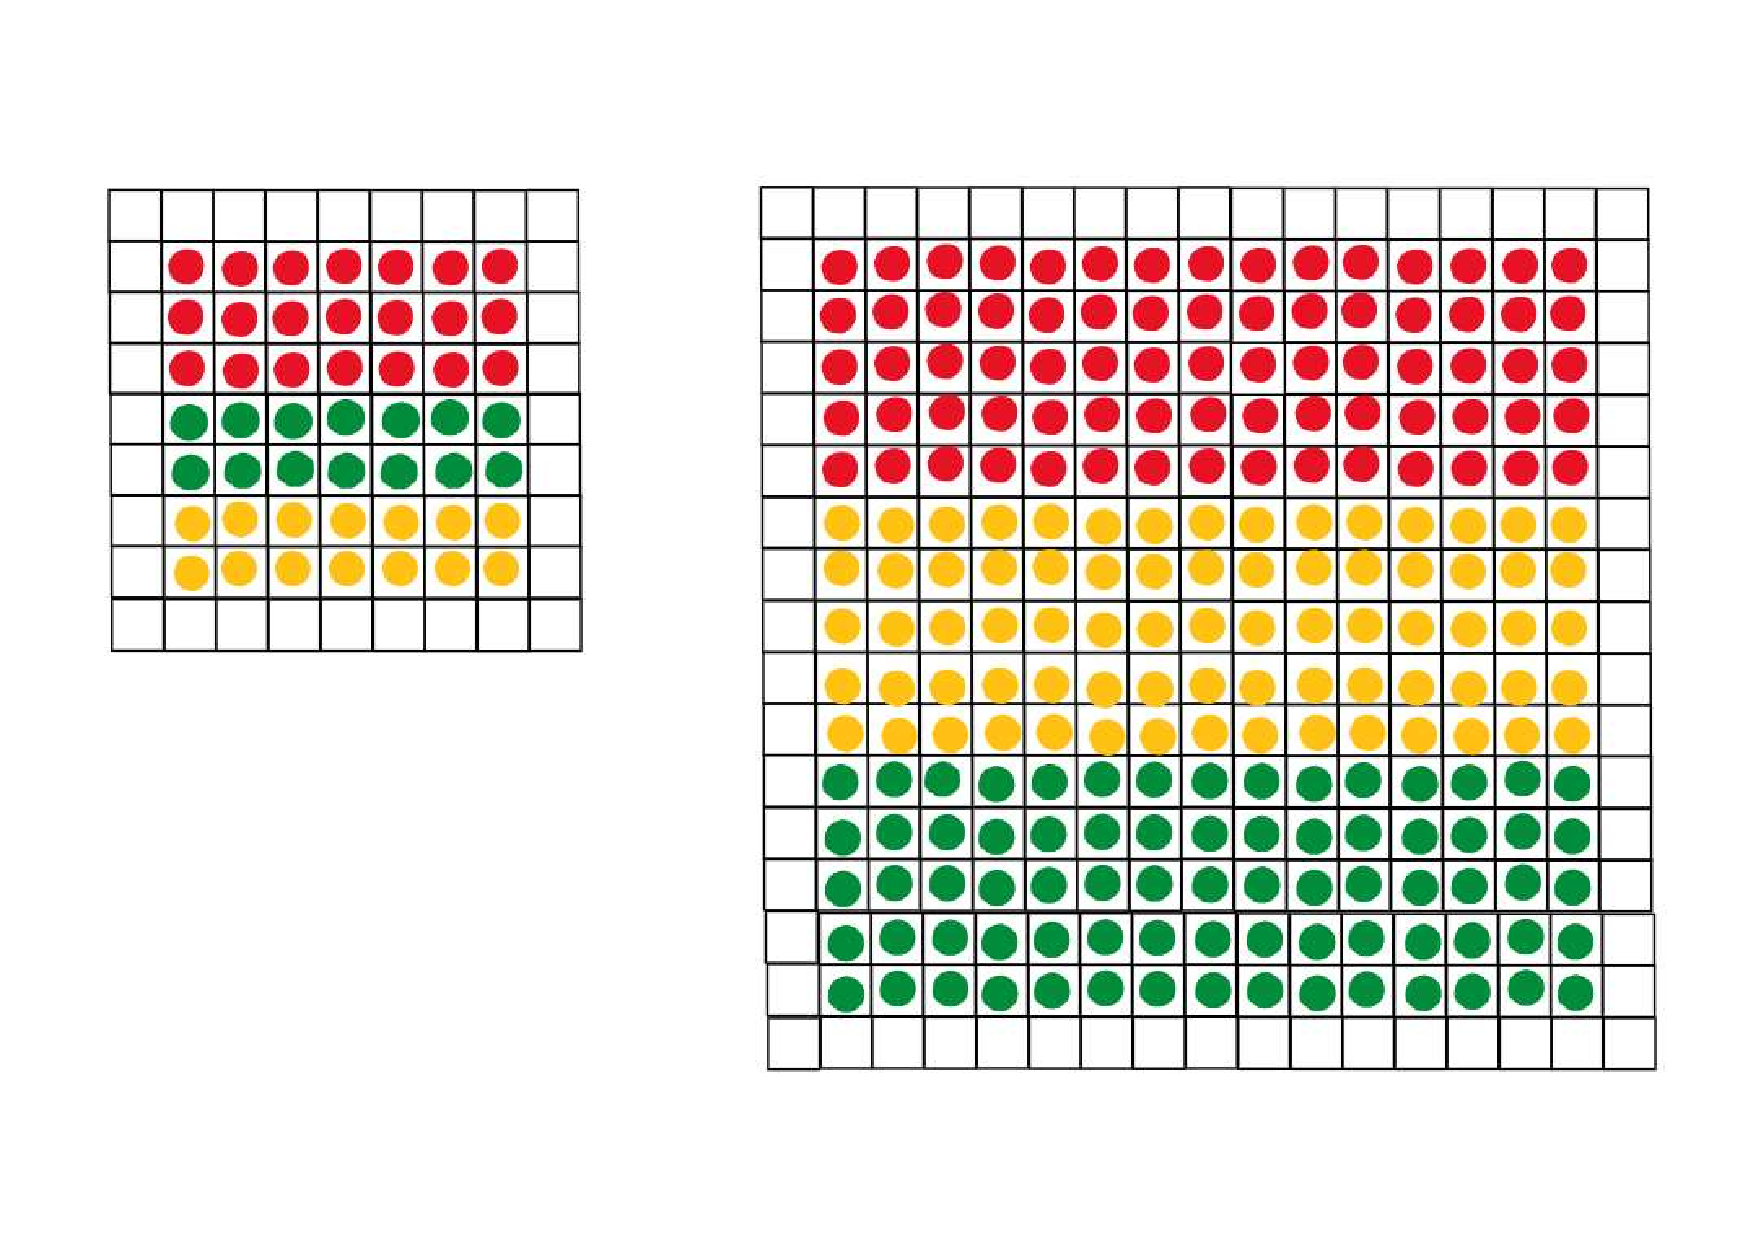
\includepdf[pages=-]{Blatt_04_01_3.pdf}
\end{document}
